\section{Evaluation}
\label{sec:evaluation}

\subsection{Setup}

We have evaluated our implementation in an environment consisting on two
computers located in the same Gigabit Ethernet network.  We run the Broker,
Third Party and one Subscriber on the first computer, and all the Publishers in
the second computer.  We perform all the analysis on the performance of several
operations in the Broker and Third Party, which run together in a computer
running Arch Linux (kernel 4.8.17-grsec) with an Intel Core i7-6600U CPU with
16GB of RAM.  In order to isolate the performance influence of the Broker and
the Third Party, we have serialized the garbling and evaluation of the garbled
circuit operations, mimicking the situation in which the Broker and Third Party
are run on different servers.

Since the Broker and the Third Party are running on the same computer, we won't
observe the delay introduced by transferring the garbled circuit over a
physical network.  For this reason we obtain an estimation of the time required
to send the garbled circuit by simulating a transmission over a Gigabit
bandwidth network.  Since we know the size of the garbled circuit, we can
easily compute the time required to transfer it over a Gigabit connection and
add that delay to the measured time.

In all our measured times, sending includes the marshaling and unmarshaling of
the garbled circuit and associated data structures necessary for transmitting
it from the Third Party to the Broker via RPC.

\subsection{Microbenchmarks}

We have selected 5 numerical operations of varying complexity (\emph{summation,
multiplicatory, mean, variance, minimum/maximum}) to evaluate the cost of the
different parts of our implementation.  We securely evaluate these functions
over the values (encoded as 32 bit fixed point numbers) received from a
variable number of Publishers.

% Plots
\begin{figure*}
    \centering
    \begin{subfigure}[b]{0.32\textwidth}
        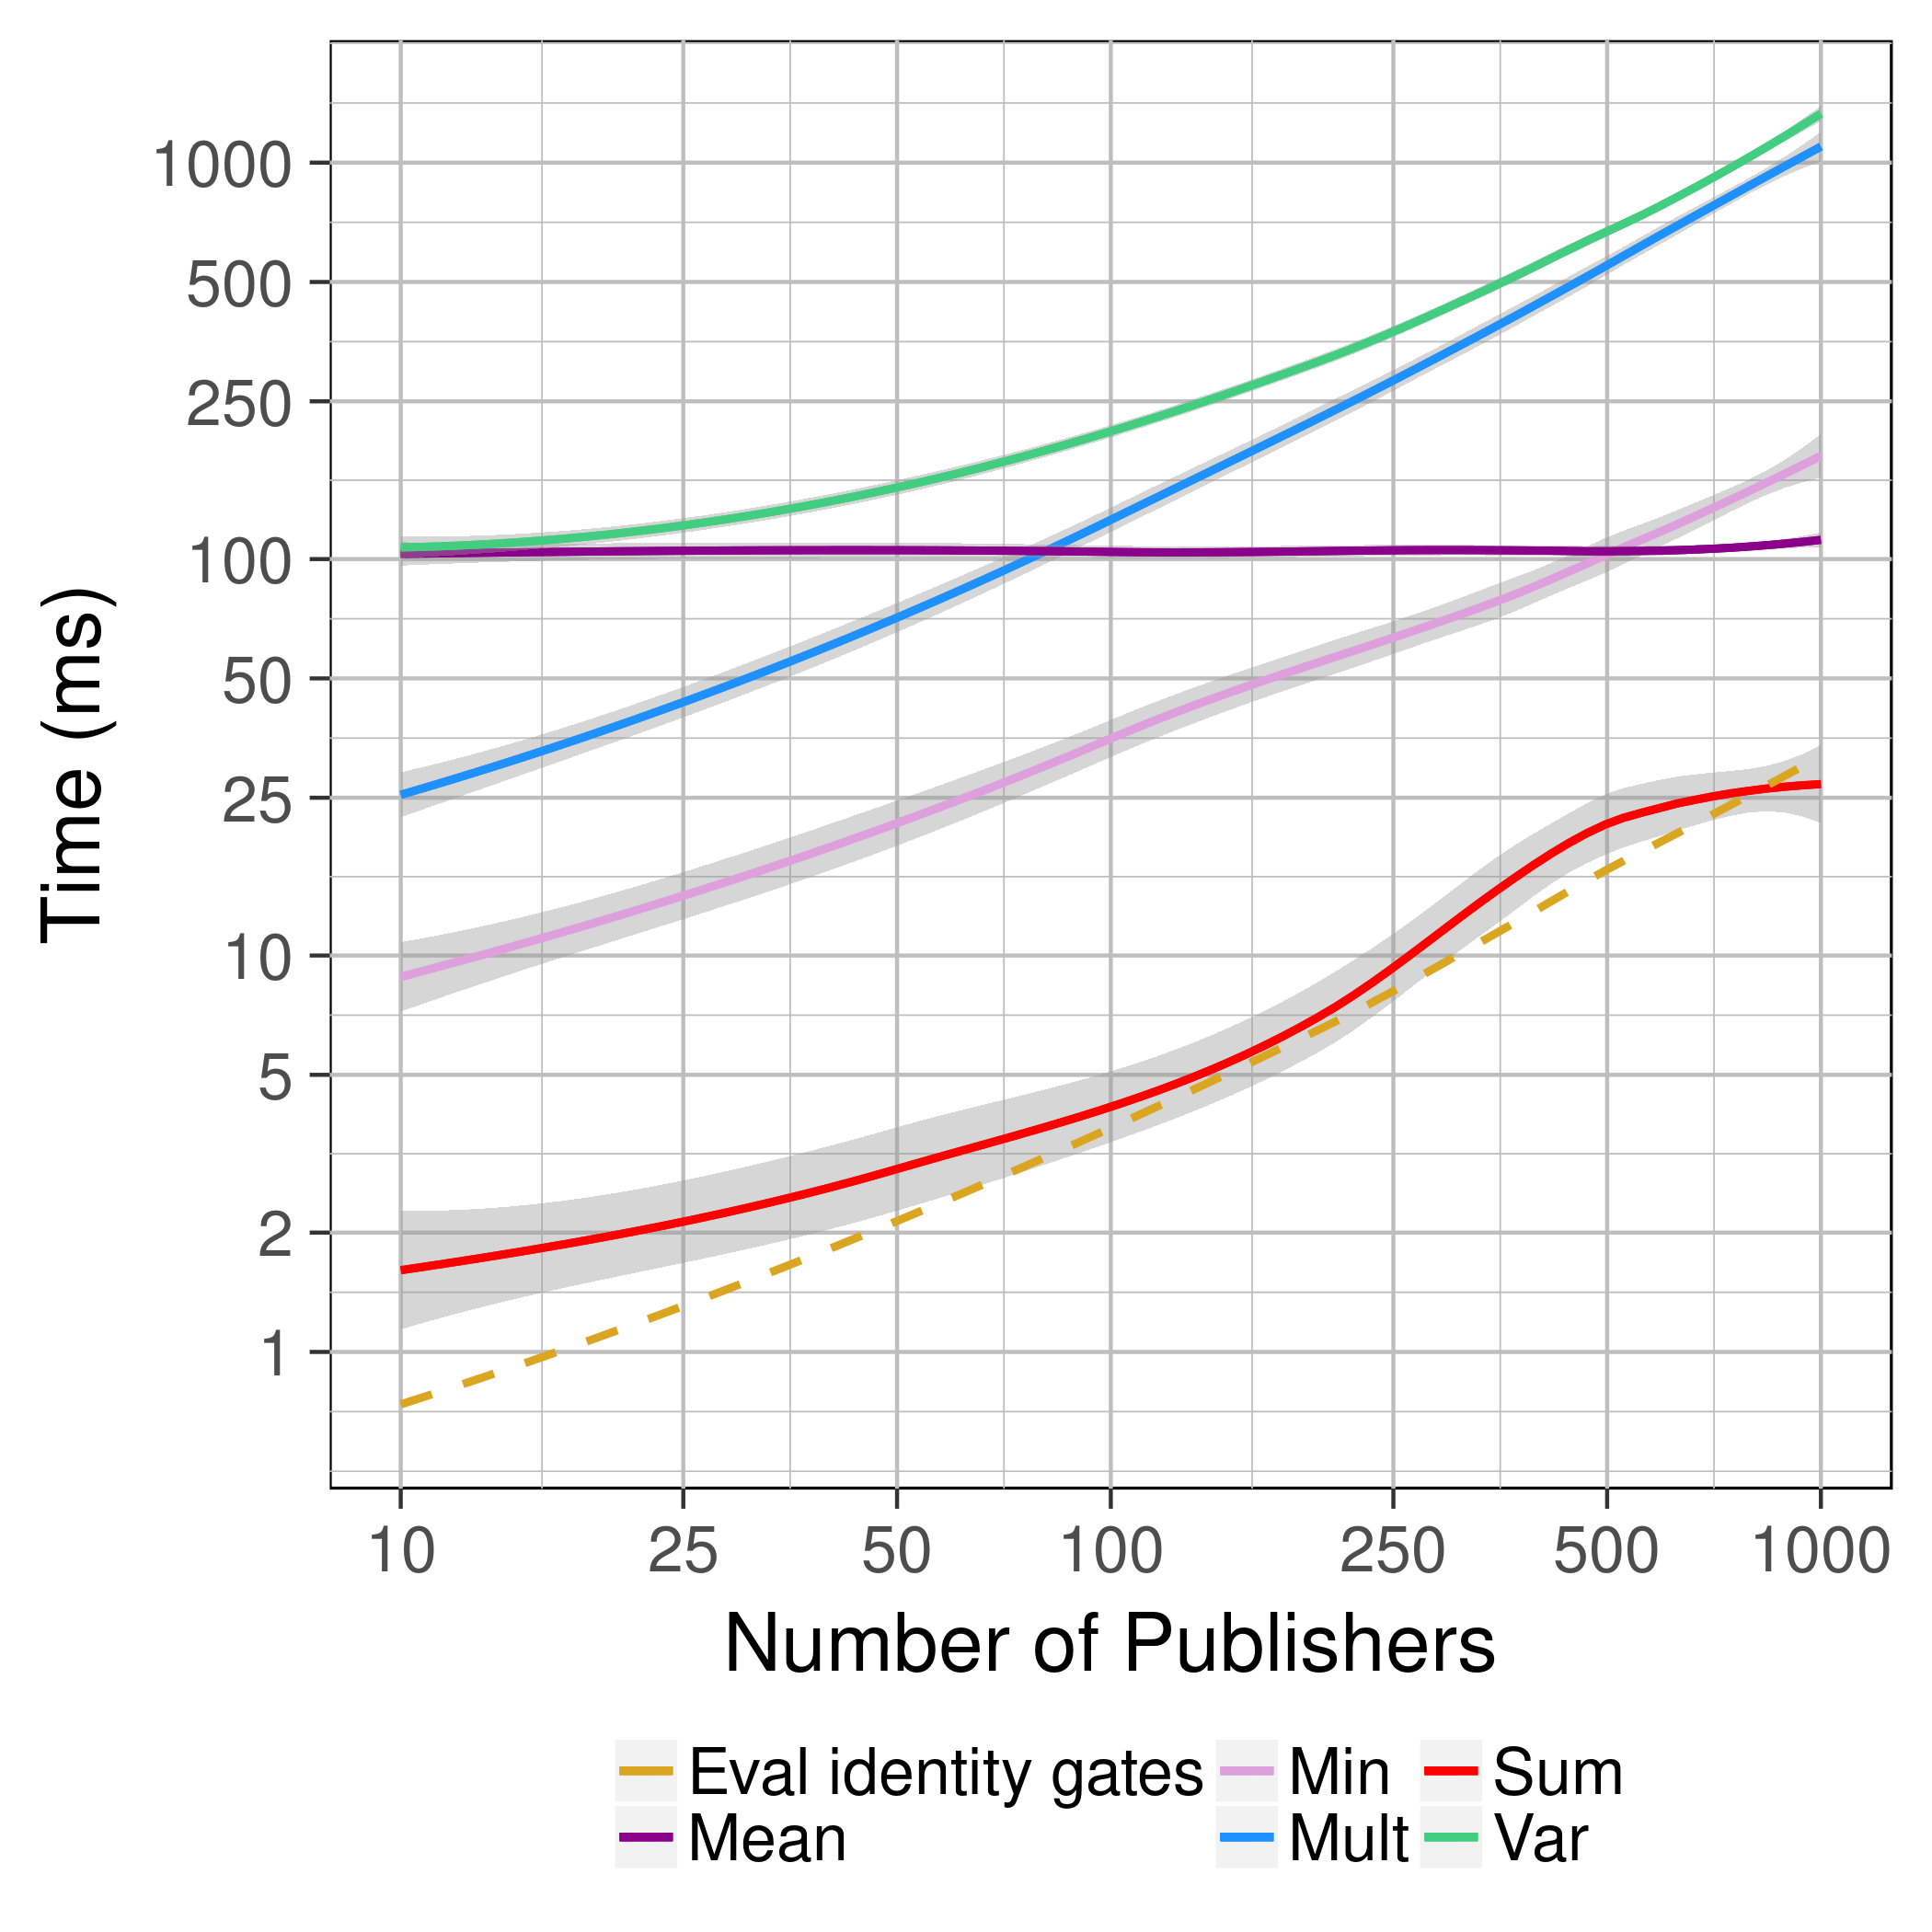
\includegraphics[width=\textwidth]{plots/garble_loglog.png}
        \caption{Garble}
        \label{fig:micro-garble-time}
    \end{subfigure}
    ~ %add desired spacing between images, e. g. ~, \quad, \qquad, \hfill etc.
    \begin{subfigure}[b]{0.32\textwidth}
        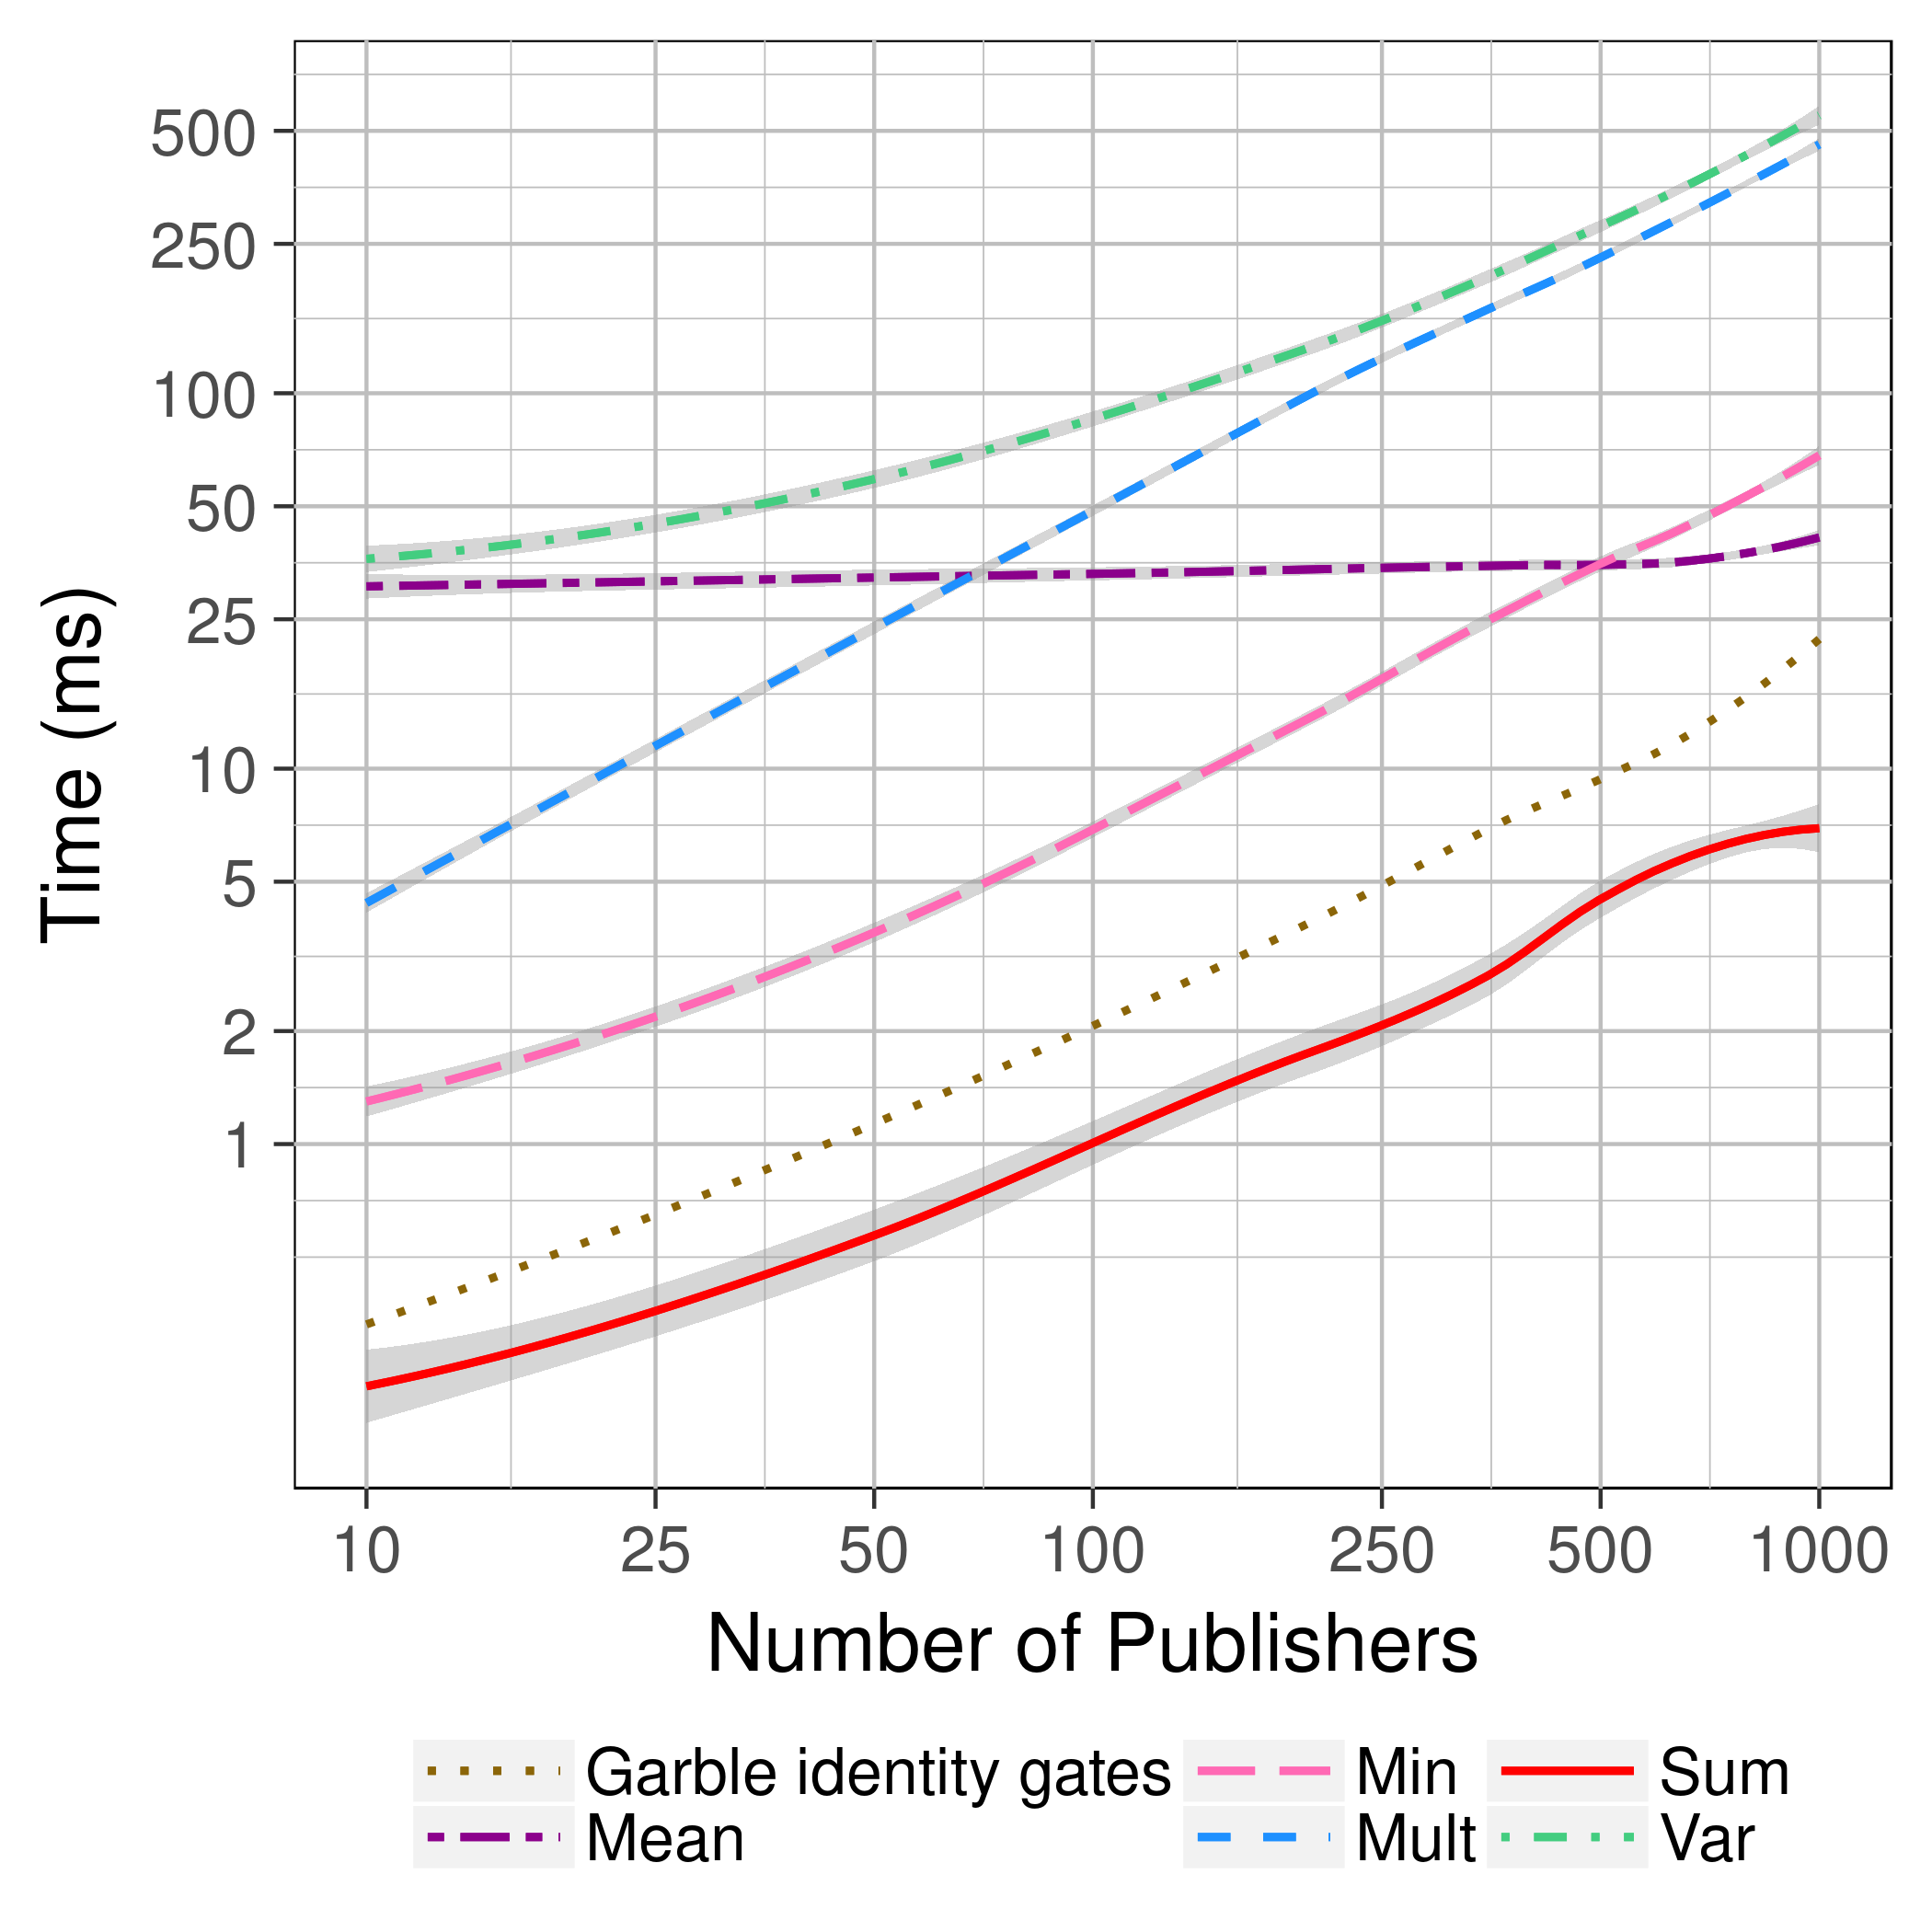
\includegraphics[width=\textwidth]{plots/eval_loglog.png}
        \caption{Evaluate}
        \label{fig:micro-eval-time}
    \end{subfigure}
    ~ %add desired spacing between images, e. g. ~, \quad, \qquad, \hfill etc.
    \begin{subfigure}[b]{0.32\textwidth}
        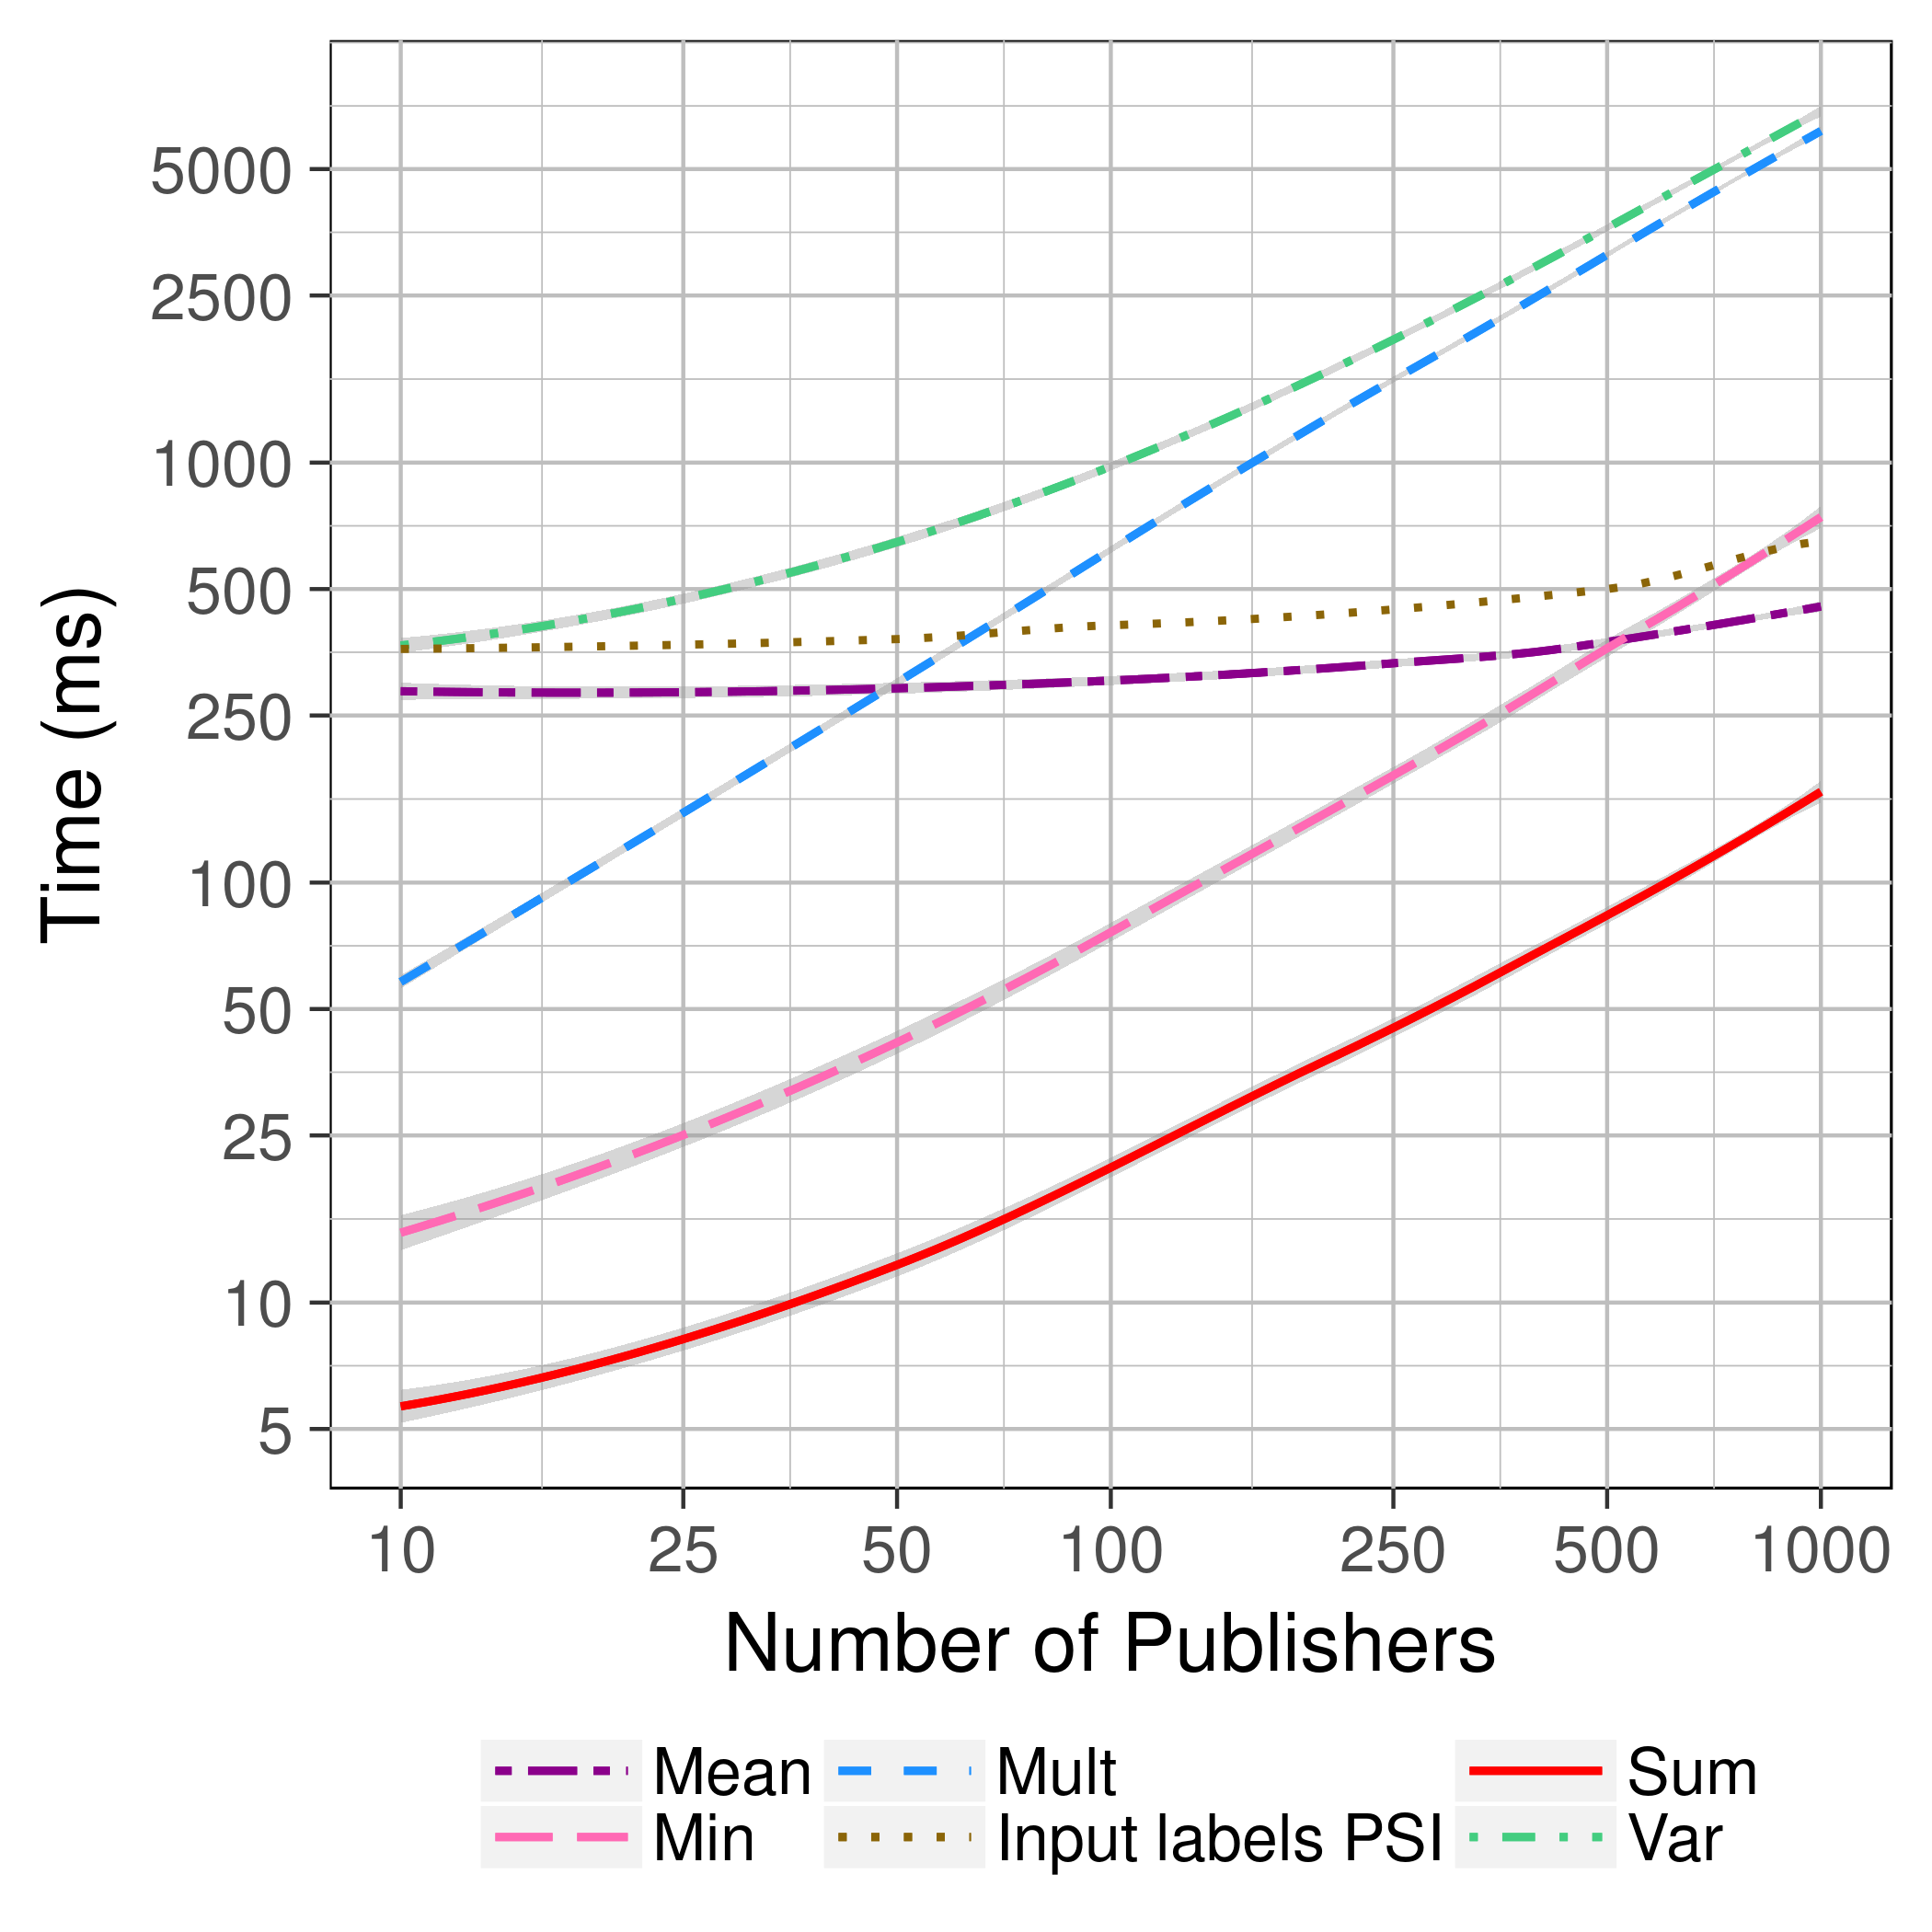
\includegraphics[width=\textwidth]{plots/send_loglog.png}
        \caption{Send}
        \label{fig:micro-send-time}
    \end{subfigure}
    \caption{Mean time required for garbling, evaluating and sending the
      garbled circuit to the Broker for each function in the microbenchmark.
      Results obtained from the mean of 5 repetitions for each configuration,
      with the confidence interval of 95\% shown in gray.}
    \label{fig:micro-times}
\end{figure*}

\begin{table}
    \begin{tabular}{l|*{4}{c}c}
      & \textbf{Sum} & \textbf{Mult} & \textbf{Mean} & \textbf{Var} & \textbf{Min/Max} \\
    \hline
    \textbf{Reduction} & 06.63 \% & 09.76 \% & 06.87 \% & 09.68 \% & 14.47 \% \\
    \end{tabular}
    \caption{Number of gates reduction for each microbenchmark function we
      would obtain by using the half-gates optimization.}
    \label{stats-times}
\end{table}

\begin{figure}
  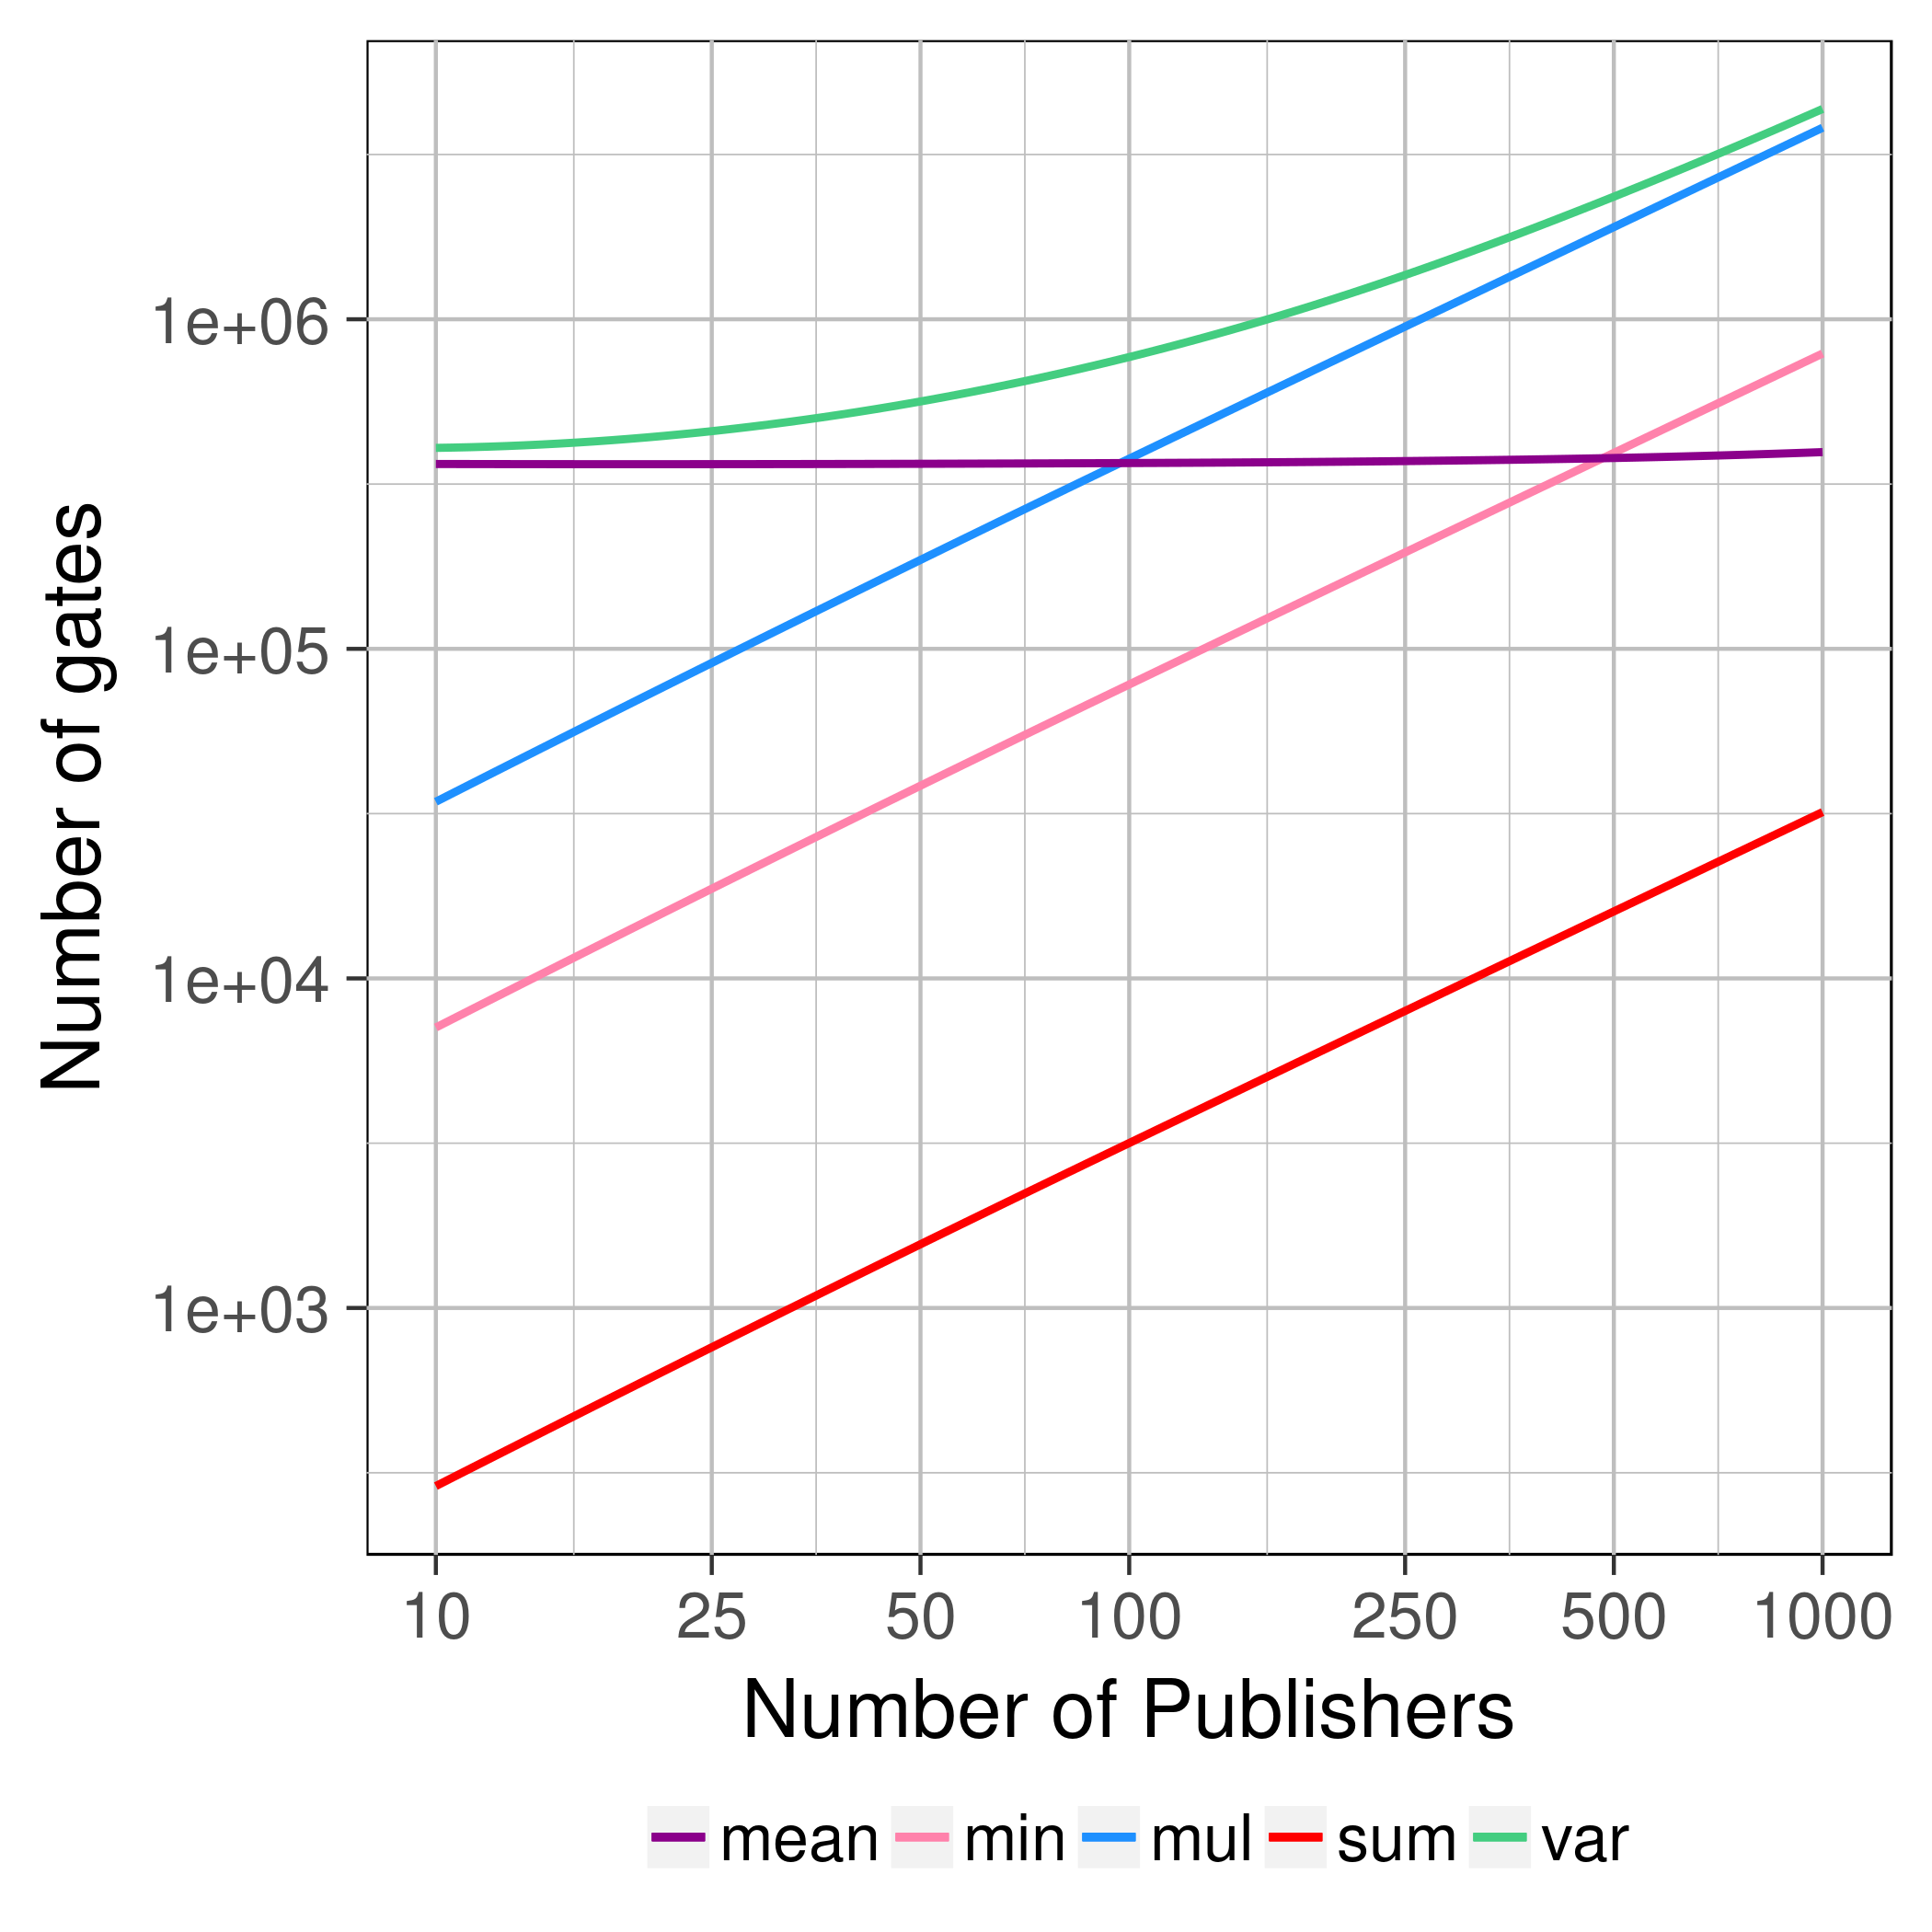
\includegraphics[width=0.38\textwidth]{plots/nonxor_gates_log.png}
  \caption{Non-XOR gates count per function used in the microbenchmarks.}
  \label{micro-nonxor}
\end{figure}

\begin{figure}
  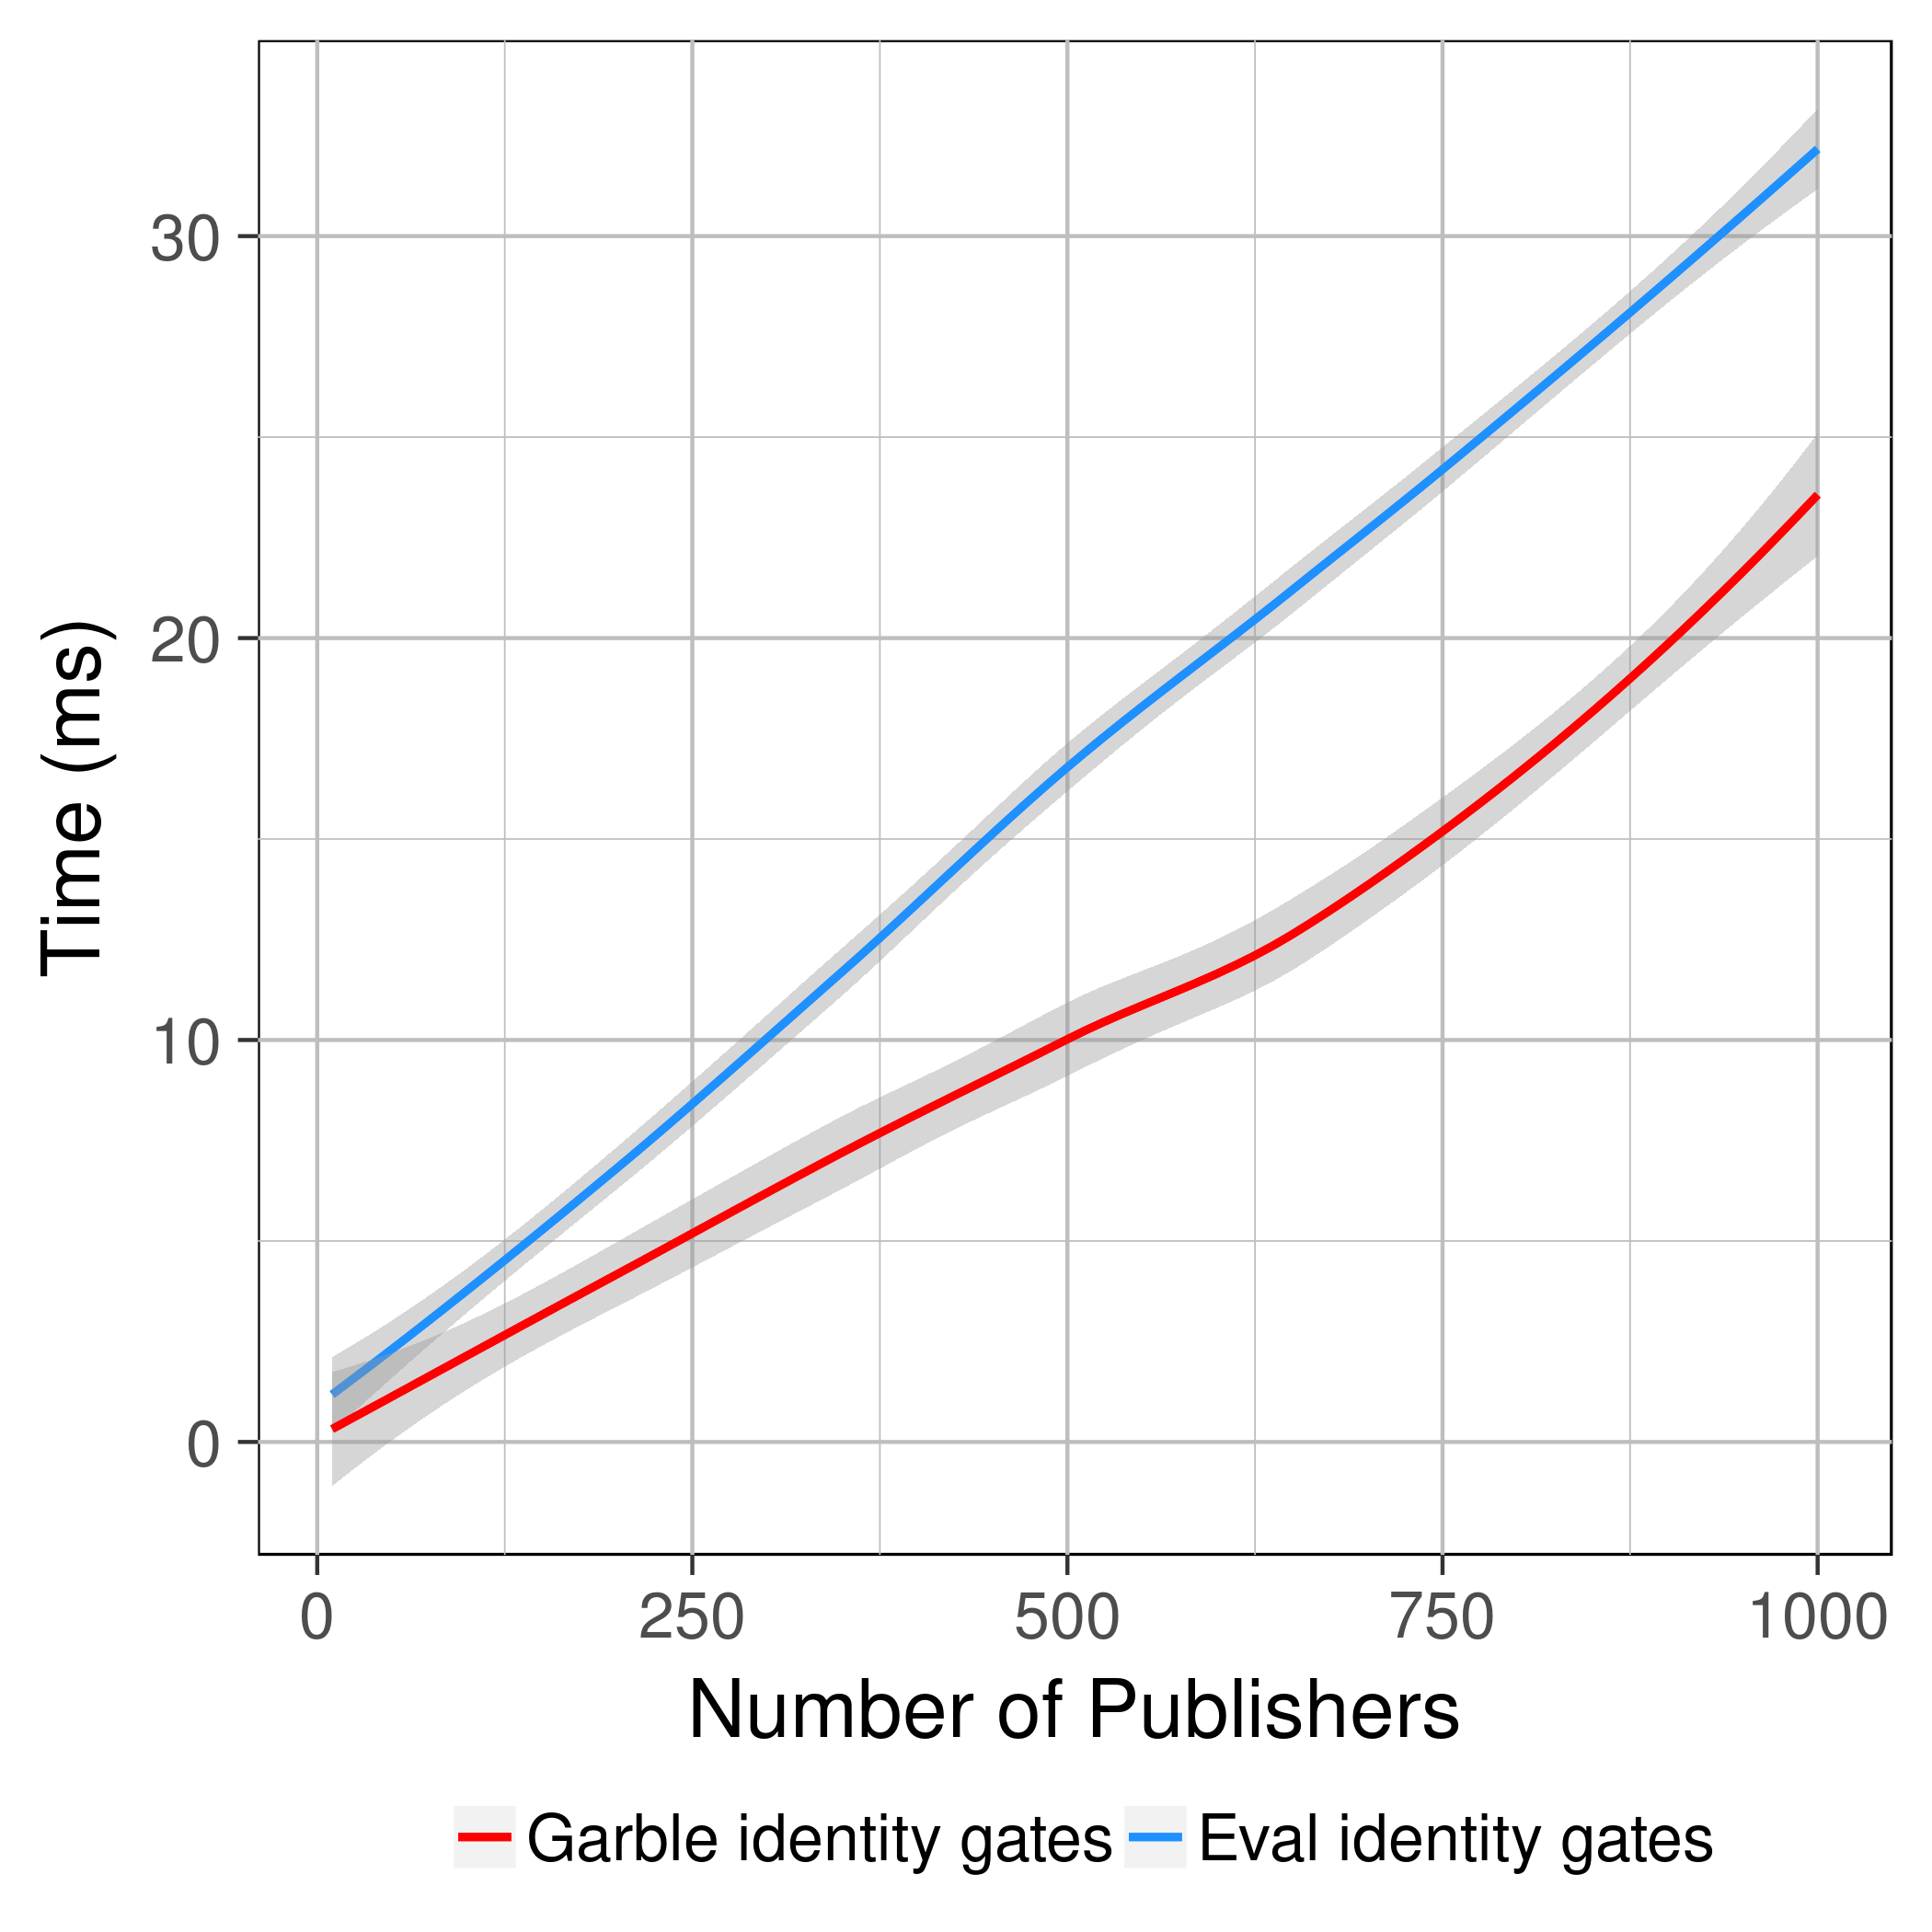
\includegraphics[width=0.38\textwidth]{plots/enc_dec.png}
  \caption{Time spent garbling and evaluating the identity input gates.
    Results obtained from the mean of all microbenchmark functions with 5
    repetitions each, with the confidence interval of 95\% shown in gray.}
  \label{micro-inputs}
\end{figure}

\begin{figure}
  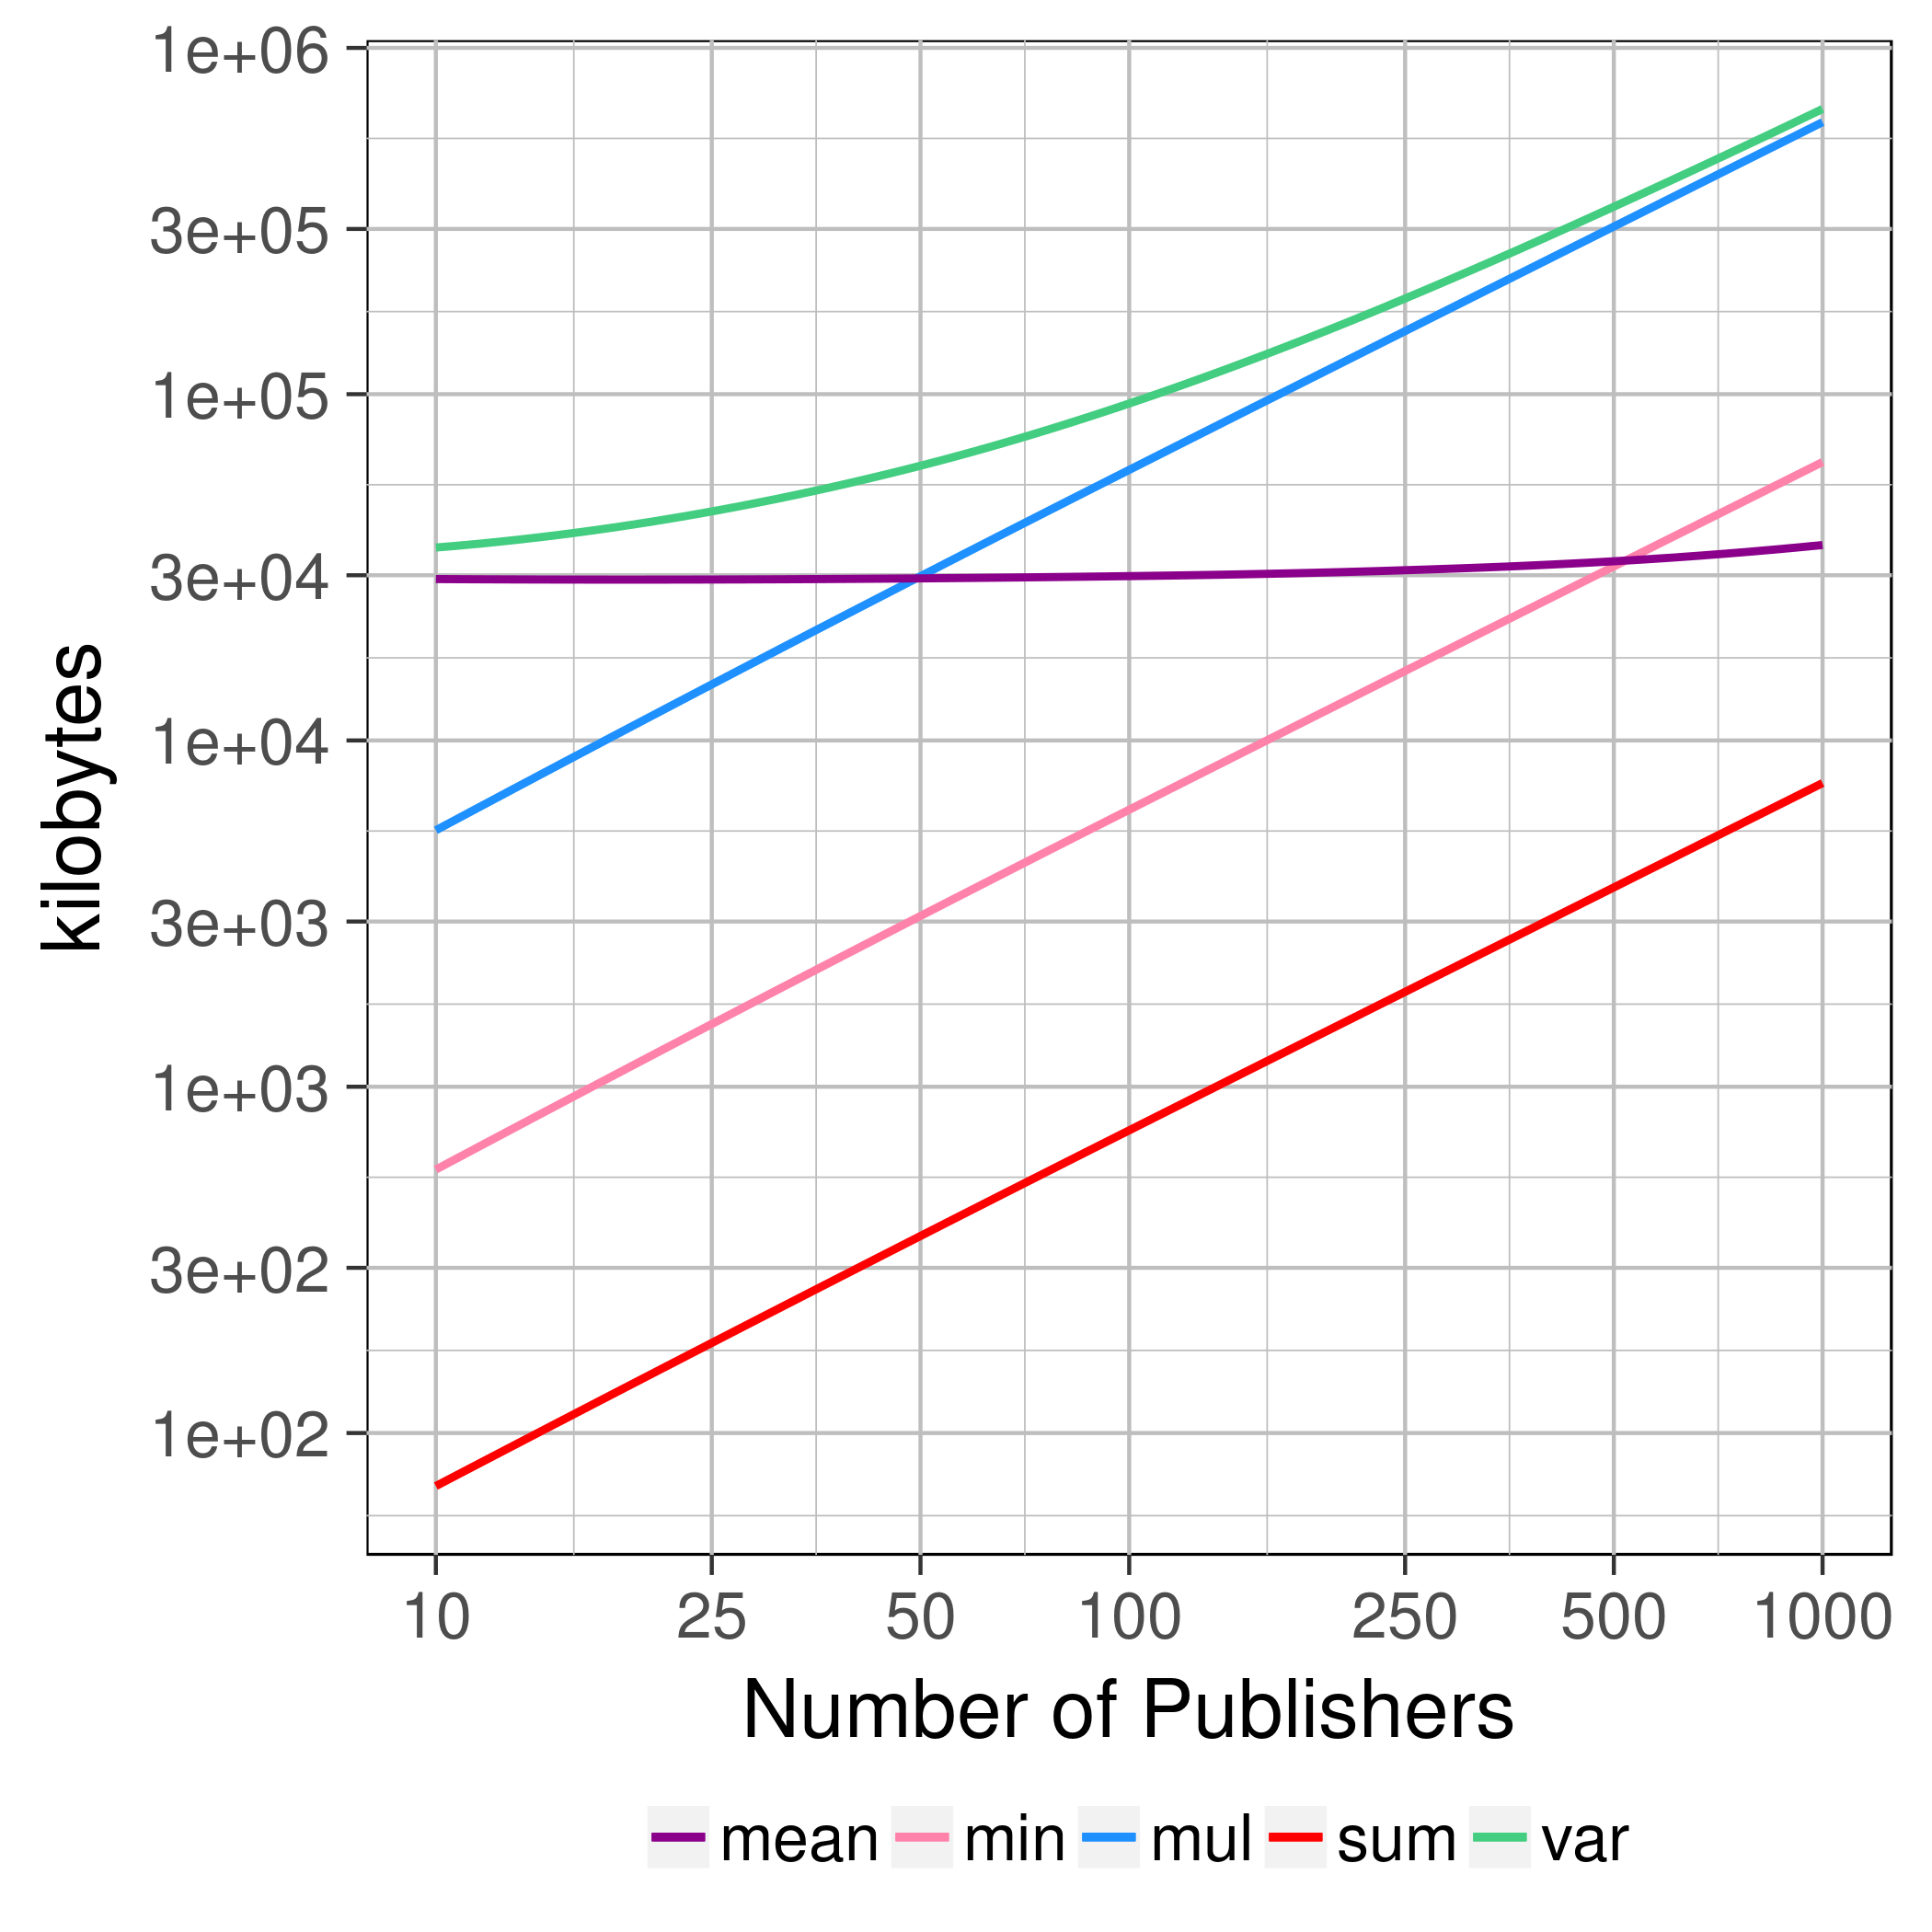
\includegraphics[width=0.38\textwidth]{plots/size_log.png}
  \caption{Size of the garbled circuit and the associated date required by the
    Broker to evaluate it.}
  \label{micro-sizes}
\end{figure}

We can see that the time spent encrypting and decrypting the inputs (that is,
garbling and evaluating the input identity gates) makes a significant influence
in the mean, min/max and sum microbenchmark, being comparable in magnitude to
the evaluation and garbling time (notice that for sum, the input
encryption/decryption time is even higher than the garbling/evaluation time).
We attribute this behavior to the fact that this part of the protocol is
implemented in go instead of C like the garbling and evaluation.

\subsection{Applications}

% Turonet, wireless propagation constant, linear regression
\paragraph{Linear regression}

% One dimensional linear regression

% Questions: How many data points to use?

% This was my original interpretation.  Since we already have the experiments,
% let's move this to the Environmental Berkeley indoor sensing data, but leave
% the formula description and linear regression explanation here.
In this application we are interested in learning the linear model of two data
streams generated by Publishers.  In particular, we perform a linear regression
so that we can model one variable (comming from one stream) as a linear
combination of another variable (comming from another stream): $y = ax + b$.
To estimate the parameters of the one dimensional linear model we use the
ordinary least squares technique, which gives us the following closed-form
formula:

\[
\begin{pmatrix} b \\ c \end{pmatrix} =
\left( \displaystyle\sum_{i=1}^n \begin{pmatrix} 1 \\ x_i \end{pmatrix}
  \begin{pmatrix} 1 & x_i\end{pmatrix}\right)^{-1}
\left( \displaystyle\sum_{i=1}^n y_i \begin{pmatrix} 1 \\ x_i \end{pmatrix}\right)
\]
\bigskip

Evaluating the formula requires an inversion of a $2 x 2$ matrix, which we perform
by following the analytic solution.

We evaluate the cost of computing the one-dimensional linear regression over
two streams with a varying number of samples.

In this application's scenario, we assume that each sensor would be an
individual Publisher that sends readings periodically.  The Broker would
accumulates streams of published values from each sensor, and when requested,
the it would samples pairs of those streams at random over a specific period of
time to perform a correlation analysis between the two.  For our experiments we
vary the number of samples and simulate the application by supplying the Broker
with the given number of samples in a batch.

%  Say you have 20 nodes in the network. There are then at most 20*19
% different links (some of these may not have any measurements because they
% may be too far). For each active link at each time we will get a
% measurement of the received signal strength in dBm (over time there is some
% fluctuation due to fading). And for each link let's say that we know the
% pairwise distance in meters.
% 
%   If you do a scatter plot of RSS in dBm versus log10(distance), then the
% resulting points will look roughly linearly decreasing. The slope of this
% line is -10*eta where eta is the path loss exponent we want to estimate
% (typically around 2.2 or so).
% 
%   So the goal is to do regression over these points and generate a running
% estimate of the slope (which may vary over time as fading may be a
% non-stationary process) based on some window of measurements from each link.
% 
%  If you want to just emulate this process, what you would really have is 20
% different publishers, each publishing the RSS from the 19 other nodes and
% also the distance between them (technically, that doesn't really change so
% doesn't need to be published/sent over and over; but we could do that just
% to be simple). The computation is take the resulting 380 pairs of points
% and do a regression to determine the slope of the best fit line.
% 
%   Time permitting, it may be helpful to see how this scales as we go from
% N=20 nodes to 40, 60, 80, 100 nodes.

% > Okay, then I'll simulate an experiment where the Publishers initially
% > send N-1 distances to the Broker, which would be stored for a day or
% > something (not indefinitely because then we loose forward secrecy), and
% > then they keep sending the N-1 signal strength periodically.

% TODO: Evaluate (analytically) the bandwidth of the Publishers, which are
% sending N-1 values per epoch each one.

\begin{figure}
  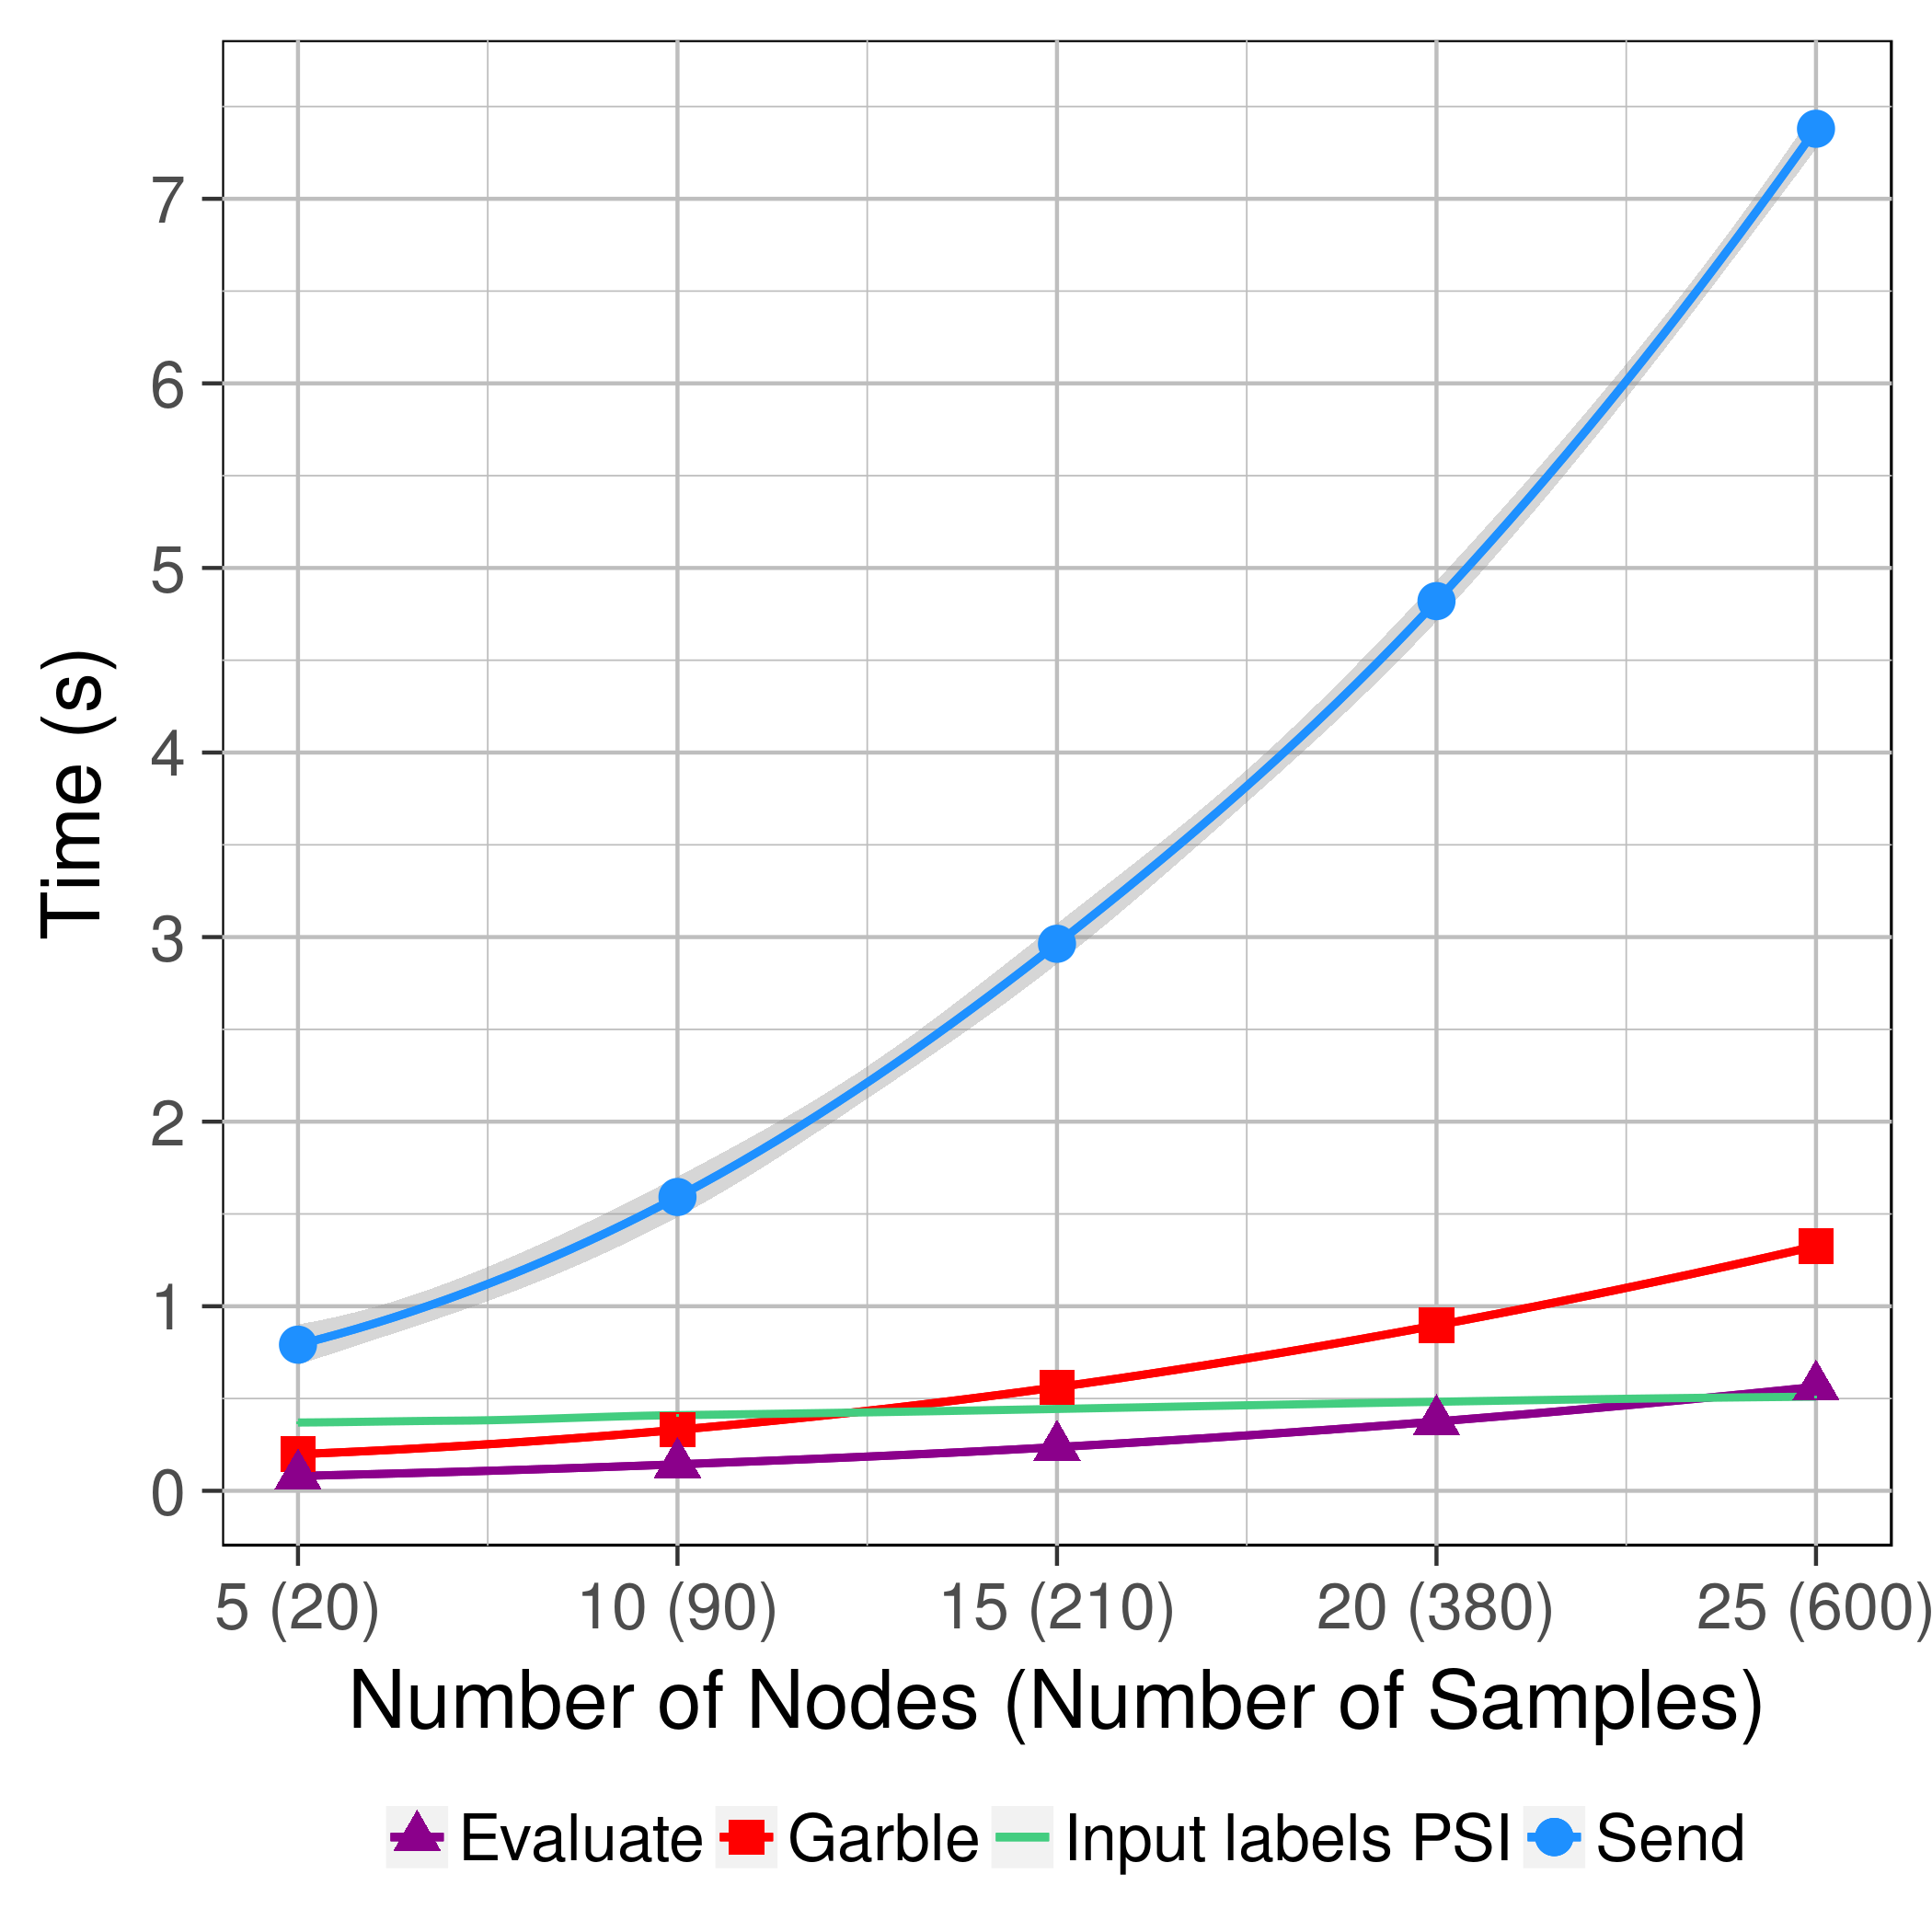
\includegraphics[width=0.38\textwidth]{plots/turonet.png}
  \caption{TODO turonet.  Results obtained from the mean of 5 repetitions for
    each configuration, with the confidence interval of 95\% shown in gray.}
  \label{turonet-times}
\end{figure}

% At 30 Nodes, we are dealing with 30*29 = 870 samples to perform the
% correlation, which corresponds to a garbled circuit of size bigger than 1
% GiB, and hit a limit on the encoding used when marshaling the garbled circuit
% in the go RPC implementation, which doesn't support data structures bigger
% than 1 GiB.

% Environmental Berkeley indoor sensing data, correlation
\paragraph{Correlation}

% The dataset provides 2.3 million readings collected from sensors with the
% following values: temperature (degree Celcius), humidity (0-100%), light
% (Lux: 0-100000), identified by sensor ID.

\footnote{\url{http://db.csail.mit.edu/labdata/labdata.html} (accessed 2017-05-18)}

% Ideas: correlation temperature~humidity, temperature~light.

Similarly to the linear regression application, in this application we have the
same scenario with sensors acting as Publishers sending a periodic stream of
reads.  Again, for our experiments we simplify the setting by supplying the
Broker with a specific number of samples in a batch.  We evaluate the cost of
the operation by varying the number of samples as before.

% Formula:
The correlation is a measure of statistical relationship among pairs of
variables, which higher value representing higher dependence.  Following the
Pearson's product-moment coefficient, we can measure the dependence between
samples of two variables (in our case, sensor readings) using the following
closed-form formula:

\[
r_{xy} = \frac{\displaystyle\sum_{i=1}^n (x_i - \bar{x}) (y_i - \bar{y})}
{\sqrt{\displaystyle\sum_{i=1}^n (x_i - \bar{x})^n (y_i - \bar{y})^n}}
\]
\bigskip

To improve efficiency, we evaluate the squared correlation ($r_{xy}^2$) to avoid
computing the square root in the function circuit, which would be an expensive
operation.

\begin{figure}
  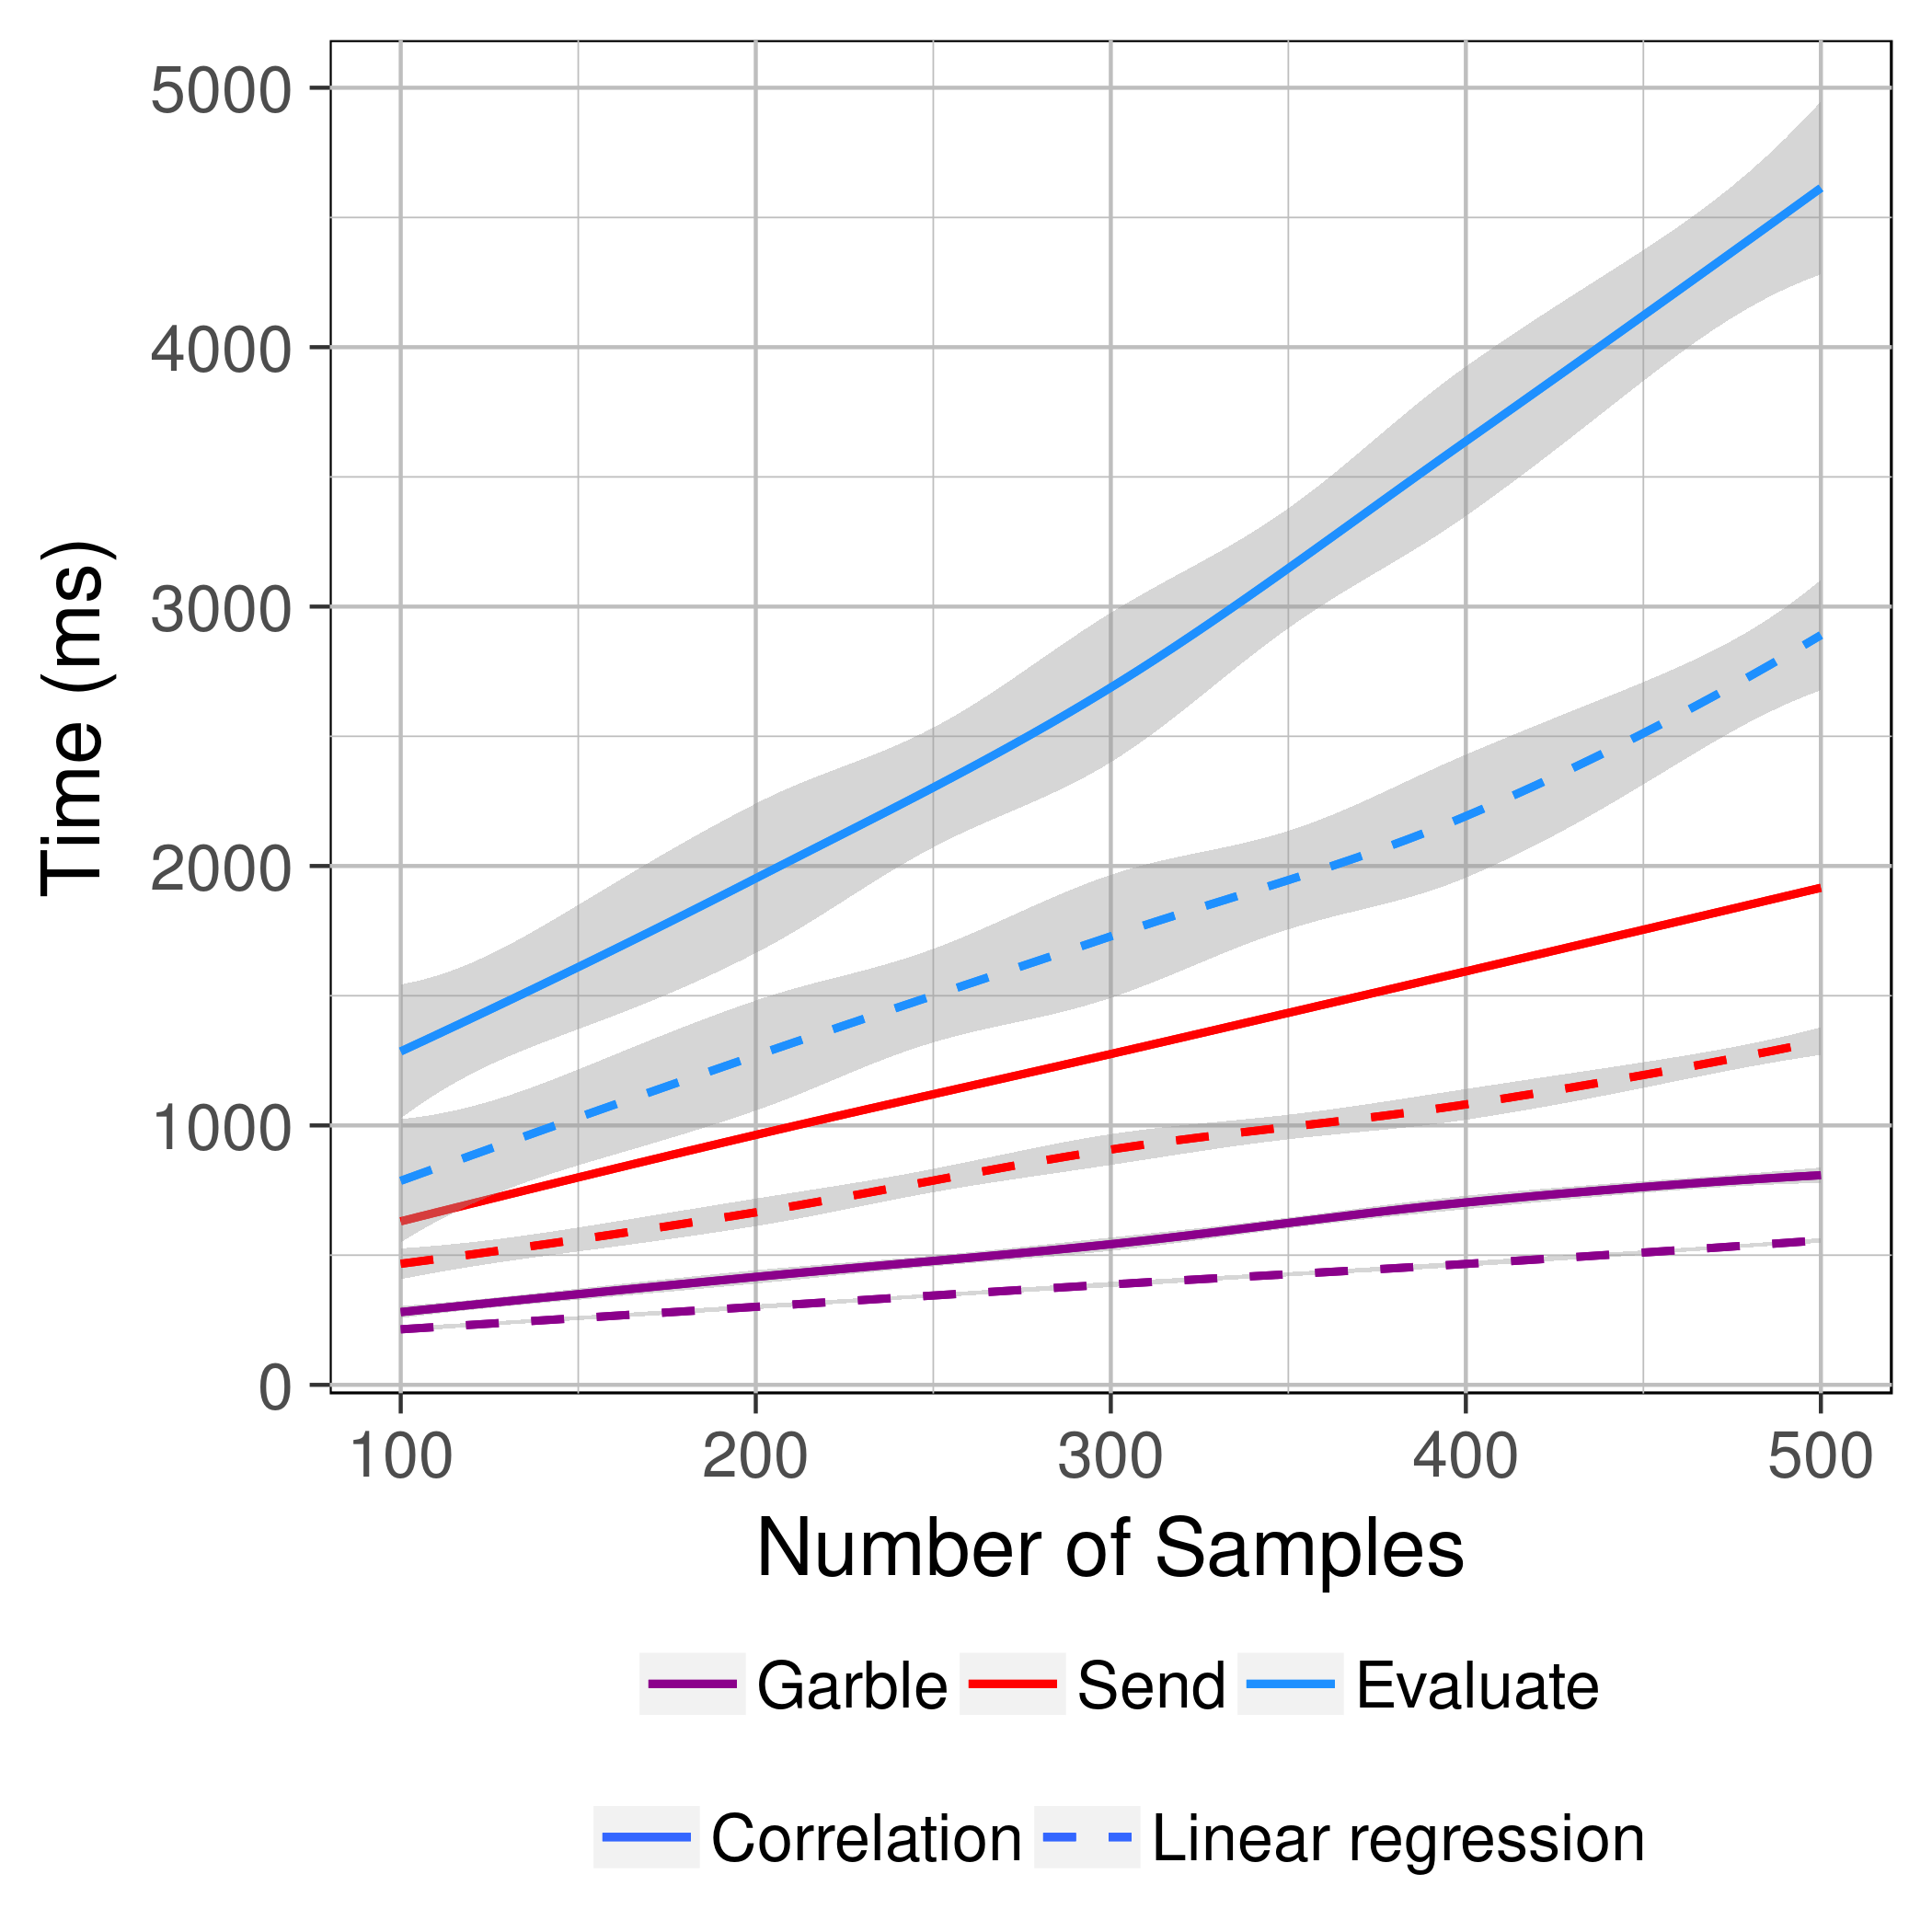
\includegraphics[width=0.38\textwidth]{plots/stream.png}
  \caption{Mean time required for garbling, evaluating and sending the garbled
    circuit to the Broker for computing the correlation and linear regression
    of data streams.  Garbling and evaluating includes the time to garble and
    evaluate the input identity.  Results obtained from the mean of 5
    repetitions for each configuration, with the confidence interval of 95\%
    shown in gray.}
  \label{stream-times}
\end{figure}

% LAX parking lot dataset, statistics
\paragraph{Continuous statistics of incoming data}

\footnote{\url{https://data.lacity.org/dataset/Los-Angeles-International-Airport-LAX-Parking-Lots/dik5-hwp6} (accessed 2017-05-18)}

% The dataset provides at a frequency of every 5 minutes and for every one of
% the 9 parking lots: total, occupied and free parking spaces.
% That's 288 values per day per parking lot.

% Privacy: Avoid revealing parking lot data at fine granularity, only reveal
% statistics of the data accumulated throughout the day.  Don't reveal data of
% individual parking lots, only combined data (except for the lot with
% more/less free spots)

Setting: We have 9 Publishers, one for each lot, which send data (current
number of free spots, current number of used spots) every 5 minutes.  The
Broker accumulates the data of a day and computes the statistics.  This
happens once per day.

% Daily statistics (used spots): mean, max, min, var of the number of cars in all the lots combined.
% Daily statistics (free spots): The marking lot which had more free spots, and the one
% that had less on average during the day.

% Time garble and time eval includes the time spend encrypting and decrypting
% the input values.

\begin{table}
    \begin{tabular}{l*{3}{r}r}
    \textbf{Statistic}  & \textbf{Garble} & \textbf{Send} & \textbf{Evaluate} & \textbf{Size} \\
    \hline
    Mean       & 199.8 ms & 461.7 ms & 98.7  ms & 45.0 MB \\
    Max/Min    & 163.3 ms & 345.2 ms & 84.9  ms & 32.3 MB \\
    Variance   & 500.7 ms & 2376.3 ms & 236.1 ms & 222.4 MB \\
    \hline
    Rank free  & 121.3 ms & 181.0 ms & 67.5 ms & 17.0 MB \\
    \end{tabular}
    \caption{Mean time required for the different steps of the protocol to
      evaluate different statistical measures of the parking lot dataset.
      Garbling and evaluating includes the time to garble and evaluate the
      input identity.  Results obtained from the mean of 5 repetitions for each
      configuration, with the confidence interval of 95\% shown in gray.}
    \label{stats-times}
\end{table}

% SKIP: 3. Road Volume sensor traffic, evaluation of the expected time to follow a path
%\paragraph{Estimation of time required to follow a path with traffic}
% http://rtmap.metro.net/ <- Not working (2017-05-15).

% SKIP: 5. Smart bill, monthly electricity bill with different cost per hour of the day / threshold.

% TODO: Discussion: bottlenecks.

As expected, the time spent sending the garbled circuit from the Third Party to
the Broker is the most expensive part of the protocol, and thus is the current
bottleneck.  This means that the quality and bandwidth of the network
connection between the Broker and the Third Party is of critical importance.

The garbling and evaluation of the identity gates could be optimized by
incorporating the operations in the C code of libgarble.  Even though the
golang implementation of the AES encryption and decryption functions use the
Intel AES-NI hardware instructions, conversions from byte vectors to AES blocks
and vice versa slow down the operation.  On the other hand, libgarble works
natively with 128 bits data types (the size of an AES block) by using the Intel
SSE2 extensions, thus not requiring any conversion during
encryption/decryption.
